\section{SECH 3: Public Key SECH}
The \ac{SECH} 3 variant is based on \ac{HPKE}.
\subsection{Motivations and Deployment Scenarios}

While we have described a mechanism to provide scalable access
to the \ac{AEAD}-based \ac{SECH} 2 design,
the access is based on either gossiping, which entails
additional coordination between clients, 
or a bootstrap step, which adds round trips and potentially sticks out.
We can avoid both of these problems with a \ac{HPKE}-based design.

In this design a client gains access by acquiring the public \var{SECHConfig}
value, e.g. via \ac{DoH}.
Also, in order to achieve the channel-level \ac{PC}
we can deploy \ac{SECH} 3 such that the \var{SECHConfig} is
only known to registered clients.

The major downside of the \ac{HPKE}-based design is that the
\ac{HPKE} \var{enc} value,
which is accessible to on-path attackers,
is distinguishable from a uniformly random value.
By observing many connections an attacker can leverage
this break \ac{PC}.

\subsection{Design}

A server produces an \var{SECHConfig} which specifies a \ac{HPKE} cipher suite
(\ac{KEM}, \ac{HKDF}, and \ac{AEAD} IDs),
a public key for the \ac{KEM}.
The server also maintains the corresponding private key for the public key.
For simplicity in this specification we assert that the \ac{HKDF}
and \ac{AEAD} are chosen at \var{SECHConfig}-compilation time.
This is unlike \ac{ECH} where the \ac{HKDF} and \ac{AEAD} are
negotiated for each session.

A client has to securely obtain the \var{SECHConfig} in order to offer \ac{SECH} 3 in a \ac{CH}, e.g. using \ac{DoH} or by any other secure and confidential means.

The client first produces the \var{ClientHello} as would be done normally
for \ac{TLS} 1.3 up to the point of computing the \ac{PSK} \var{binder}.

The client instantiates a \ac{HPKE} context using the suite specified in
the \var{SECHConfig} and produces a 32 octet \var{enc}.
As of writing the only \ac{KEM} with a 32 octet \var{enc} by the \ac{IANA} is
the \ac{X25519} \ac{EC}\ac{DHE}.
The \var{enc} is produced by generating a 32 octet random key, $k$, and then encrypting
that key with the public key from the \var{SECHConfig}.
The \var{random} field is set to the value of \var{enc}.

The \var{sech\_inner\_random} is defined in Listing~\ref{lst:sech5-inner-random}.

\begin{listing}
    \begin{Verbatim}[frame=single]
k = RAND_bytes(32) // for client
enc = HPKE-encap(k, pubkey)
k = HPKE-decap(enc, privkey) // for server
sech_inner_random = HKDF-Expand-Label(
    k, // secret
    "sech inner random", // label
    "", // context
    32) // output length
    \end{Verbatim}
    \captionsetup{width=.8\linewidth} 
    \caption[SECH 3 Inner Random]{\label{lst:sech5-inner-random}Computation of the \var{sech\_inner\_random} in \ac{SECH} 3. The client generates $k$ randomly computes \var{enc} using the server's public key. The server decapsulates $k$ from \var{enc}. The \var{HKDF-Expand-Label} function is defined Section~7.1 of RFC 8446 \citep{rfc8446}.}
\end{listing}


The client concatenates the inner servername and inner \ac{ALPN} list separated by a null byte, and pads this to 16 bytes with 0s. Call the resulting string \var{sech\_cleartext}.
The client creates \var{ClientHelloOuterAAD} which is a clone
of the \ac{CH} but with the \varlegacysessionid{} field set to 0s,
and the \var{binders} list truncated off.
Using the \ac{AEAD} specified in the \var{SECHConfig} the client encrypts
\var{sech\_payload} with \var{ClientHelloOuterADD} as \ac{AAD}
producing a 32 octet ciphertext \var{sech\_cipher}
(including the 16 byte \ac{AEAD} tag). 
For simplicity we assert in this draft that only \ac{AEAD}s with a 16 byte tag are valid in an \var{SECHConfig}.

% [ ] client encrypts the \var{padded\_servername} with the AEAD specified in SECHConfig, and with key $k$ and a \nonce which is the first 12 octets of the hash of \var{SECH5ClientHelloAAD}, and with \var{SECH5ClientHelloAAD} as AAD, producing \var{sech5\_cipher} which is the concatenation of the encrypted text and the tag $t$

% [ ] \var{SECH5ClientHelloAAD} is the \var{ClientHello} but with the portion in which the AEAD cipher (encrypted text and tag) will be placed set to zero, the size and location of this region depends on \var{SECHConfig}

% [ ] \var{SECH5ClientHelloAAD} is the \var{ClientHelloOuter} but with the \var{random} and \var{legacy\_session\_id} set to all 0s

The client encodes \var{enc} and \var{sech\_cipher} in the \var{random} and \var{legacy\_session\_id} fields producing a partial \ac{CHO}
(excluding the \var{binders})
as depicted in Figure~\ref{fig:sech5-cover}.
If the client is using a resumption \ac{PSK} controlled by the backend server
the \var{binders} list is computed
using the synthetic \var{ClientHelloInner} transcript rather
than the transcript of \var{ClientHelloOuter}.


\begin{figure}[H]
\centering
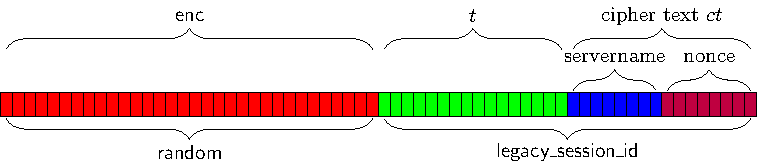
\includegraphics[width=\linewidth]{figure/sech5-cover.pdf}
\captionsetup{width=.8\linewidth} 
\caption[SECH 3 Cover]{Placement of the \ac{SECH} 3 \var{enc} and \var{sech\_cipher} in the 64 byte cover of the \ac{CH}.}
\label{fig:sech5-cover}
\end{figure}

The \var{ClientHelloInner} has the \var{random} field replaced with \varsechinnerrandom{}, and the first 16 bytes of the
\varlegacysessionid{} replaced with \var{sech\_payload}.
Also, the extension data field of the outer \ac{SNI} is set to all 0s.

The client-facing server attempts to decapsulate \var{enc} with the private key associated with \var{SECHConfig} retrieving $k$; on failure 
the client-facing server continues with normal TLS 1.3,
although implementations should ensure that the timing of the response in case of \ac{SECH}
decryption failure is not distinguishable from the case when
\ac{SECH} succeeds.
Using the \ac{HKDF} in \var{SECHConfig} $k$ is transformed into \varsechinnerrandom{}.

% [ ] TODO: Unlike \ac{ECH} we do not support arbitrary numbers \var{SECHConfig}s on the server
% in order to ensure the server response time is consistent and does not reveal \ac{SECH}
% decryption success or failure. 

The client-facing server computes \var{ClientHelloOuterAAD} and the \nonce, and then attempts to decrypt and retrieve \var{sech\_payload}; on failure  
the client-facing server continues with a normal TLS 1.3 handshake.

On success the client-facing server constructs \ac{CHI} by replacing 
the first 16 bytes of \ac{CHO}'s \var{legacy\-\_session\-\_id}
with \var{sech\_payload}, and also replacing the \var{random} field
with \var{sech\_inner\_random}.
Also the \var{extension\_data} of the \var{server\_name} extension is set to all 0s.

The client-facing server forwards \var{ClientHelloInner} to the backend server.
The backend server processes this message, detecting the all-zero \ac{SNI} extension value,
and decodes the inner \ac{SNI} and \ac{ALPN} from the \varlegacysessionid{}.

If the backend server needs to negotiate different parameters by sending a
\var{HelloRetryRequest} this message is constructed as in normal \ac{TLS} 1.3,
at which point \ac{SECH} is abandoned.
The remaining messages are just performed to not stick out,
and the outer parameters of the subsequent \ac{CH2} are used.

In the case that no \var{HRR} is triggered the backend server can continue to signal
its acceptance of \ac{SECH}.
The \ac{SH} contains a special \var{sech\_accept\_confirmation} value in the first 24 octets of the \var{random} field,
which has the same definition as in \ac{SECH} 2 (see Listing~\ref{lst:sech2-accept-function}), except the label value is ``sech 3''.

The handshake continues as specified in RFC 8446, except that \ac{CHI} is used in the transcript instead of the \ac{CHO},
and the selected identity should correspond to the inner servername.


\section{Implementation Notes}
We have completed an implementation of an earlier draft of
our \ac{SECH} 2 design in a fork of the OpenSSL codebase\footnote{The tag for our implementation at the time of submission: \url{https://github.com/Neimhin/openssl-sftcd-fork/tree/DissertationSubmission}}.
During implementation of that draft we discovered several protocol vulnerabilities
which we have
rectified in the specification provided above,
but this means that the implementation lags behind the specification.

In particular, work left to be done in order to provide a simple prototype of the above \ac{SECH} 2 specification includes:
\begin{itemize}
    \item Correctly account for maximum \ac{SECH} payload length.
    \item Provide an \ac{API} for setting the \ac{ALPN}.
\end{itemize}

As with \ac{SECH} 2, we have implemented an earlier draft of \ac{SECH} 3 which was vulnerable to
various attacks.
After discovering those attacks we rectified the design resulting in the above \ac{SECH} 3 specification.

Our implementation still lags behind our \ac{SECH} 3 spec. In particular, the following aspects are still not implemented.
\begin{itemize}
    \item Derivation of \var{sech\_inner\_random} and insertion of same into the \ac{CHI}.
    \item Client verification of the acceptance confirmation signal.
    \item \ac{API} for \ac{ALPN}.
\end{itemize}

Our implementation so far adds 6 new \ac{API} methods:
\begin{enumerate}
    \item \var{SSL\_CTX\_set\_sech\_inner\_servername}: (client only) to set the inner servername.
    \item \var{SSL\_CTX\_set\_sech\_symmetric\_key}: (client and server) to set the \varsechlongtermkey{}.
    \item \var{SSL\_CTX\_set\_sech\_version}: (client and server) to choose between \ac{AEAD} and \ac{HPKE} based \ac{SECH} (version 2 or 3).
    \item \var{SSL\_get\_sech\_status}: (client and server) to query the success/failure of the \ac{SECH} attempt, as well as fetch the peer's inner servername on success.
    \item \var{SSL\_CTX\_sech\_set1\_sechconfig}: (client only) to set \var{SECHConfig} to use for \ac{SECH} 3.
    \item \var{SSL\_CTX\_sech\_server\_enable\_file}: (server only) To enable an \var{SECHConfig} and corresponding private key for \ac{SECH} 3.
\end{enumerate}

Some other features which have not yet
been implemented are:
\begin{itemize}
    \item Allowing a server to accept both \ac{SECH} 2 and \ac{SECH} 3 connections. Currently the \var{set\_sech\_version} \ac{API} only allows specifying one version.
    \item Allowing a server to enable multiple \varsechlongtermkey{}s and \var{SECHConfig}s.
\end{itemize}

\subsection{Implementation Challenges}
Although the description of our implementation is relatively short,
the OpenSSL implementation was by far the most time-consuming aspect of this project.
Here we'll discuss briefly some of the things we found difficult
in writing the implementation.

Firstly, OpenSSL uses the C programming language.
Unlike memory-managed languages like Java or Python,
memory management in C is entirely manual.
There are good reasons for using the C programming language
for implementing cryptographic libraries.
For one, C is available an almost all computing platforms,
including mobile phones, IoT devices, etc.
Secondly, secure implementations of cryptographic protocols need to account
for timing and power-consumption side-channels.
Yielding control of memory management to the language runtime
risks the introduction of such side-channels.

With that said, manual memory management leaves a lot more room for programmer error.
Mistakes can lead to memory corruption,
which can manifest as seemingly unrelated errors and/or crashes.
A couple of times during development we introduced such mistakes into the code,
and identifying the issue took a lot of painstaking debugging time.

Another thing we found challenging was the implementation
of the syntethic transcript hash for \ac{SECH}.
Our implementation ended up involving some changes to
quite low-level aspects of OpenSSL's \ac{TLS} 1.3 implementation.
Identifying the appropriate places in the code to make these changes
such that all required information was available at the right time
involved a lot of trial and error, as well as a lot of time to
understand the existing code.
Luckily OpenSSL is already equipped with an expansive test suite
which allowed us to verify that our changes did not cause breakages in any
other functionality.

\section{Testing}

We have implemented 12 basic tests of the \ac{SECH} 2 implementation and \ac{API} using the OpenSSL test infrastructure.
These tests perform \ac{SECH} 2 handshakes under various configurations to test that that the handshake succeeds/fails appropriately.

Writing tests with the OpenSSL test infrastructure has the advantage of comfortably allowing granular tests for specific errors and conditions at specific points of execution.
A disadvantage is that the tests we have written involving a client and server do not actually use the system's network and hence cannot be easily inspected with external tools like Wireshark.

The \var{test\_sech2\_roundtrip\_accept} sets up a client and shared-mode server.
The server is enabled with two certificates, one for the client-facing server and one for the backend server.
The test expects the server to return a certificate corresponding to the backend server.

The \var{test\_sech2\_roundtrip\_accept\_and\_resume\_with\_ticket} first performs the same test as \var{test\_sech2\_roundtrip\_accept} but then additionally tests that the client can reconnect to the server using a resumption \ac{PSK} derived from the first connection. This test revealed an interesting bug and design flaw during development. In an earlier design the \ac{SECH} 2 session key was derived from a transcript of the full \var{ClientHello} including the \var{pre\_shared\_key} extension. However, the \var{binder} values in the \var{pre\_shared\_key} extension are also bound to the rest of \var{ClientHello}. If the session key is bound to the \var{binder} and then used to edit an earlier part of the \var{ClientHello} then the \var{binder} is invalidated. The solution is that the session key should be derived from the \var{ClientHello} up to but not including the \var{binder}, and the \ac{SECH} 2 encryption has to take place before the \var{binder} is calculated.

We have implemented two tests of \ac{SECH} 3 using the OpenSSL unit test infrastructure.
The first performs an \ac{SECH} 3 roundtrip and checks the appropriate certificate was returned.
The second performs an \ac{SECH} 3 roundtrip
using parameters that trigger a \ac{HRR},
and expects that a \ac{tlsC} corresponding to the outer \ac{SNI} is returned, as well as
the \ac{SECH} status of the server and client indicating that \ac{SECH} was abandoned due to \ac{HRR}.

As of writing the \ac{SECH} 3 tests do not pass because the client acceptance-confirmation verification
and the inner random are in a half-implemented state.